\section{Architecture}
% Follow UWE? Mabye good? I tink it maches not baad in this case. http://uwe.pst.ifi.lmu.de/teachingTutorial.html

\begin{figure}
\centering
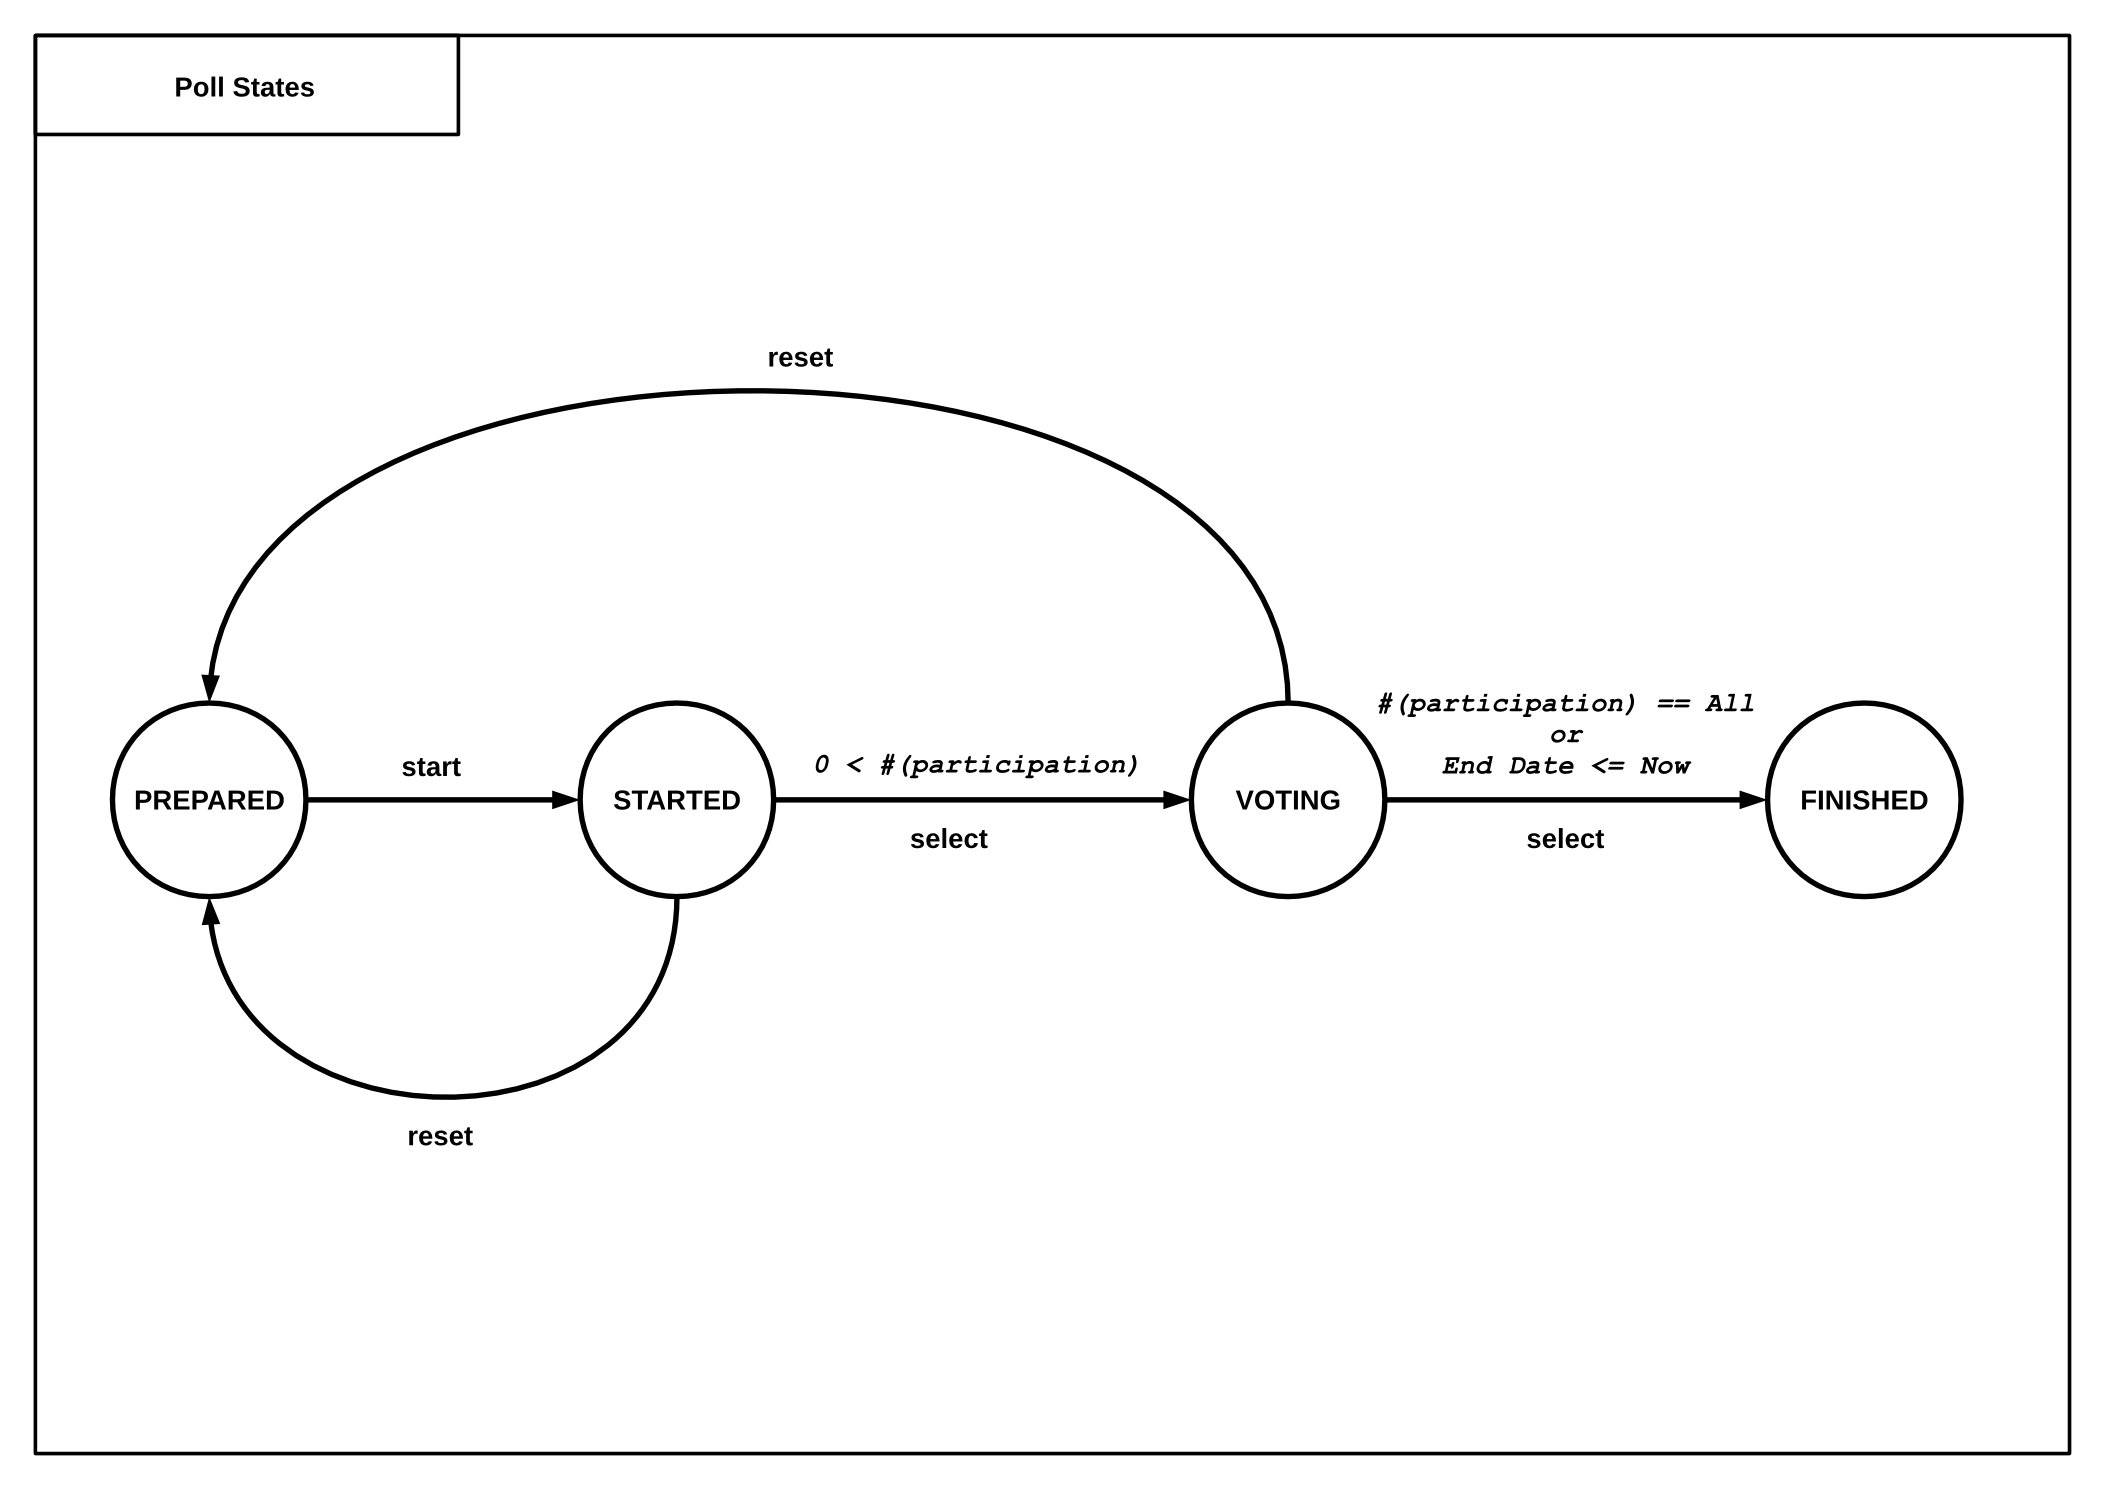
\includegraphics[width=0.9\textwidth]{png/poll-states.png}
\caption{Poll States}
\end{figure}

\subsection{Content Model}
The following view describes the systems content model. The corresponding implementation serves as backbone of the running application in form of keeping the data and persisting it. In the case of the content model, no presentation concerns are included. As well as that no behaviour is defined here. The six classes represent all essential entity types that are involved in the requirements. Two enumeration types serve as additional datatypes. 

High value comes to this view due to the fact that it can be directly be mapped on the JPA and the transfer object classes contained in the systems implementation. Apart from the fixed nature of the content model, described in the current requirements, a derivation process defining the Java classes can be of high good for further evolution and maintenance of the deployed system providing constitutive quality assurance.

\begin{figure}
\centering
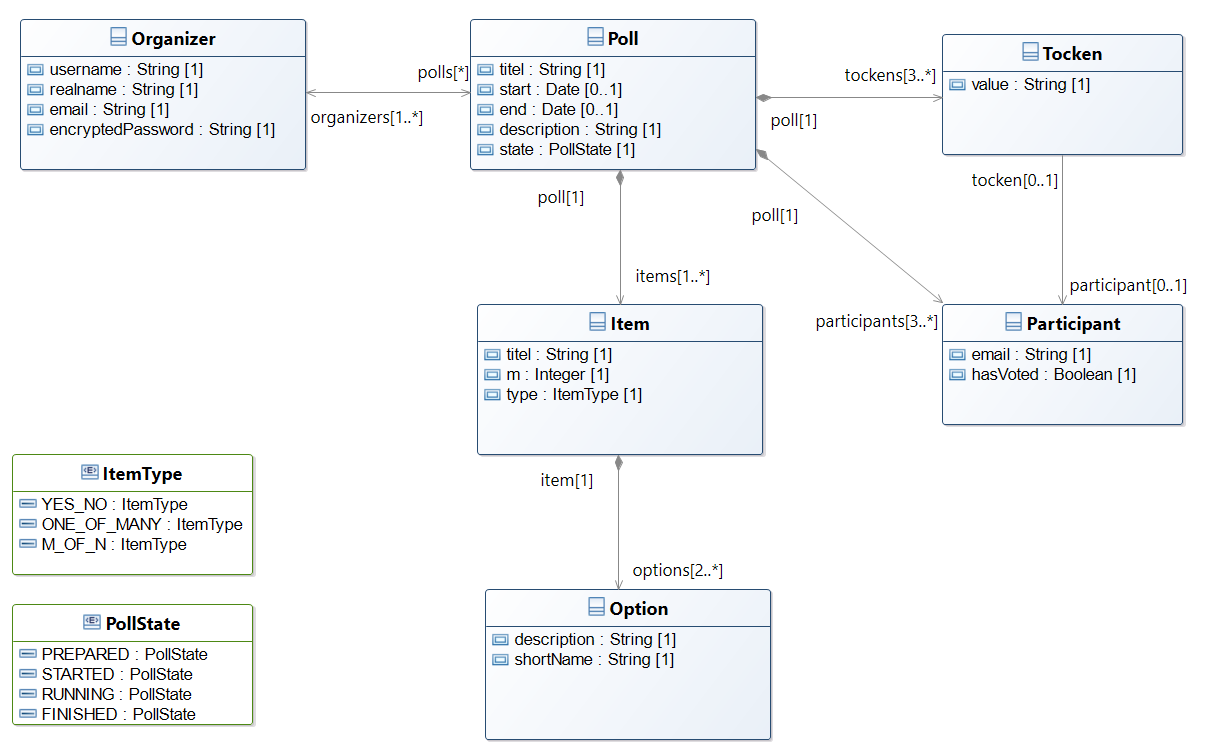
\includegraphics[width=1.0\textwidth]{png/domain_model.png}
\caption{Votes content model}
\end{figure}


\subsection{VotesEJB Architecture}
% Maybe we can call that navigation model? Enables refference on http://uwe.pst.ifi.lmu.de/teachingTutorialNavigation.html
%Mentioned by ebert in the last web engeneering course! Will make rudige cum!
\subsection{VotesWar Architecture}
% Do you mean packaging?